\documentclass[12pt]{article}
\usepackage[amsmath]{e-jc}
\usepackage{booktabs}

\dateline{TBD}{TBD}{TBD}
\MSC{68R15, 05A05}
\Copyright{The author. Released under the CC BY license (International 4.0).}

\title{Shuffle anti-squares of every even length from 24}
\author{Vamshi Jandhyala}
\authortext{}{London, United Kingdom.}

\newcommand{\zz}[1]{0^{#1}}

\usepackage{graphicx}
\begin{document}
\maketitle

\begin{abstract}
A binary word is a shuffle square if it can be split into two identical subsequences, and an even word is
a shuffle anti-square if none of its cyclic rotations is a shuffle square. Grytczuk, Pawlik and
Pleszczy\'nski found that the shortest shuffle anti-squares have length 24 and conjectured that they exist in
every even length from 24 upward. We prove this. For every $k \ge 0$ the word
$\zz{k+9}\,1\,\zz{5}\,11\,\zz{k+9}\,1\,\zz{2}\,1\,0\,111$ is a shuffle anti-square of length $2k+34$, and
the shorter lengths are covered by the family $\zz{k+5}\,1\,\zz{2}\,1111\,\zz{k+4}\,111\,0\,1111$, which is in
fact an anti-square for every $k$. The first family has a short human proof. Both families have been verified
for all $k$ in the Lean proof assistant. The proof for the first family extends to every word obtained from it
by multiplying each zero run by a constant and replacing each one by the same odd number of ones. Since one
cut can only rotate a word, some even binary words of every length from 24 need two cuts to become a shuffle
square. The same authors and Ruci\'nski found such a word of length 24 and conjectured that two cuts always
suffice; by computer this holds up to length 34.
\end{abstract}

\section{Introduction}

A word $w$ is a \emph{shuffle square} if its positions can be coloured with two colours so that the letters of
each colour, read in order, spell the same word $u$. For example, $0110$ is not a shuffle square: one copy must take the first $0$ and one of the $1$s, and spells $01$, while the other spells $10$. Its rotation $1100$ is one, with copies $10$ and $10$. The question below is whether some rotation always rescues an even word in this way. Shuffle squares were introduced by Henshall, Rampersad and
Shallit~\cite{HRS}. Deciding whether a binary word is a shuffle square is NP-complete~\cite{BV}, and He, Huang,
Nam and Thaper conjectured that almost every binary word with an even number of each letter is
one~\cite{HHNT}, and He and Post have since proved it~\cite{HP}.

Call a binary word \emph{even} if it contains an even number of $0$s and an even number of $1$s. Grytczuk,
Pawlik and Pleszczy\'nski proved that every even binary word splits into two subwords, one of which is a cyclic
shift of the other~\cite[Theorem 2]{GPP}, and conjectured that some cyclic rotation of every even binary word
is a shuffle square, having checked this up to length $20$~\cite{GPP2}. The conjecture fails at length $24$. They called an even word a \emph{shuffle
anti-square} if none of its rotations is a shuffle square, found by computer that the shortest ones have length
$24$ (there is exactly one up to rotation, reversal and exchanging the letters), listed all anti-squares of
lengths $24$, $26$ and $28$, and made the following conjecture.

\begin{conjecture}[{\cite[Conjecture 1]{GPP}}]\label{conj}
There is a shuffle anti-square of length $2n$ for every $n \ge 12$.
\end{conjecture}

We prove the conjecture with explicit families.

\begin{theorem}\label{main}
For $k \ge 0$ let
\[
U_k = \zz{k+9}\;1\;\zz{5}\;11\;\zz{k+9}\;1\;\zz{2}\;1\;0\;111
\qquad\text{and}\qquad
W_k = \zz{k+5}\;1\;\zz{2}\;1111\;\zz{k+4}\;111\;0\;1111 .
\]
Every $U_k$ and every $W_k$ is a shuffle anti-square. They have lengths $2k+34$ and $2k+24$, so
Conjecture~\ref{conj} holds.
\end{theorem}

Section~\ref{sec:runs} reduces the question to arithmetic on the runs of zeros. Section~\ref{sec:U} proves
that $U_k$ is an anti-square by hand, in a stronger form (Theorem~\ref{thm:blow}) that allows every zero
run to be multiplied by a constant and every one to be replaced by an odd block of ones. For $W_k$ the same reduction leaves a finite family of linear systems
in the parameter $k$; Section~\ref{sec:verify} describes how these were checked, including a complete
formalisation of Theorem~\ref{main} in Lean~4, and records counts of anti-squares up to length $34$.
Section~\ref{sec:cut} draws the consequence for the cutting distance of~\cite{GPP2}.

\section{Runs of zeros}\label{sec:runs}

A binary word with $m$ ones can be written uniquely as $w = \zz{e_0}1\zz{e_1}1\cdots1\zz{e_m}$; we call
$(e_0,\dots,e_m)$ its \emph{zero runs}. For example, $0110$ has zero runs $(1,0,1)$. In a shuffle square the two colour classes are the \emph{copies}.

\begin{lemma}\label{lem:split}
Let $w = \zz{e_0}1\zz{e_1}1\cdots1\zz{e_m}$ be split into two copies $A$ and $B$ that both spell $u$. Then
$m$ is even, and $u$ has zero runs $(r_0,\dots,r_{m/2})$ where, for each $j$, $r_j$ equals the number of
zeros of $A$ lying between the $j$-th and $(j+1)$-th ones of $A$, and also equals the number of zeros of $B$
lying between the $j$-th and $(j+1)$-th ones of $B$ (with the conventions that the $0$-th one is the start of
$w$ and the $(m/2+1)$-th one is its end).
\end{lemma}

\begin{proof}
Each copy spells $u$, and the zero runs of a copy are read off exactly as stated. The ones of $w$ split
equally because both copies contain the ones of $u$.
\end{proof}

We shall use the lemma for rotations of a fixed circular word. Write the circular word as a cyclic sequence of
ones separated by \emph{gaps} of zeros. A rotation is determined by a cut point on the circle; the gap
containing the cut contributes its two parts to $e_0$ and $e_m$. Each copy's zeros in a gap all lie in the
same zero run of that copy, namely the run spanning the gap.

It is convenient to merge the first and last zero runs of $u$ into a single \emph{cyclic run} $\rho_0 = r_0 +
r_{m/2}$, and to write $\rho_j = r_j$ for $1 \le j < m/2$. Reading around the circle from the cut, the
cyclic runs of $A$ and of $B$ then agree term by term. This is weaker than Lemma~\ref{lem:split}, and we use
the extra information only at the very end of Section~\ref{sec:U}: the cut lies inside the run $\rho_0$ of
both copies, and the zeros of $\rho_0$ preceding the cut number $r_{m/2}$ in both copies.

\section{The family $U_k$ and its blow-ups}\label{sec:U}

We prove a stronger statement, in which every zero run of $U_k$ is multiplied by $\lambda$ and every one is
replaced by a block of $\mu$ ones. Read around a circle, let $V = V(K,\lambda,\mu)$ consist of
\begin{gather*}
G = \zz{K\lambda},\quad P_1 = 1^{\mu},\quad g_1 = \zz{5\lambda},\quad P_2 = 1^{2\mu},\quad G' = \zz{K\lambda},\\
P_3 = 1^{\mu},\quad g_2 = \zz{2\lambda},\quad P_4 = 1^{\mu},\quad g_3 = \zz{\lambda},\quad P_5 = 1^{3\mu},
\end{gather*}
in this order. We call $G$ and $G'$ the \emph{long gaps}, $C_1 = P_1 g_1 P_2$ and $C_2 = P_3 g_2 P_4 g_3 P_5$
the \emph{clusters}, and the $8\lambda$ zeros of $g_1, g_2, g_3$ the \emph{short} zeros. Read from the start
of $G$, $V(k+9,1,1) = U_k$ (Figure~\ref{fig:circle}).

\begin{theorem}\label{thm:blow}
If $K \ge 9$, $\lambda \ge 1$ and $\mu \ge 1$ is odd, then $V(K,\lambda,\mu)$ is a shuffle anti-square.
\end{theorem}

Both conditions are needed: $V(8,1,1)$, $V(8,1,3)$, $V(9,1,2)$ and $V(9,1,4)$ are themselves shuffle
squares (explicit splittings, checked in Lean). The proof uses $K > 8$ in the mass argument and in the final
step, and the oddness of $\mu$ once, in the parity argument of Step~1. It never uses the parity of a number of
zeros, which is why $\lambda$ is arbitrary.

The proof has four steps. Comparing how the two copies share the long gaps, a mass count shows that the
run of one copy through one long gap must coincide with the run of the other copy through the other long
gap, or that one copy owns no one between them (Step~1). In the second case the fact that each copy holds
half of the zeros already gives a contradiction (Step~2). In the first case, matching the remaining runs of
the two copies index by index rules out every splitting but two (Step~3), and the position of the cut rules
out those two (Step~4).

\begin{figure}[ht]
\centering
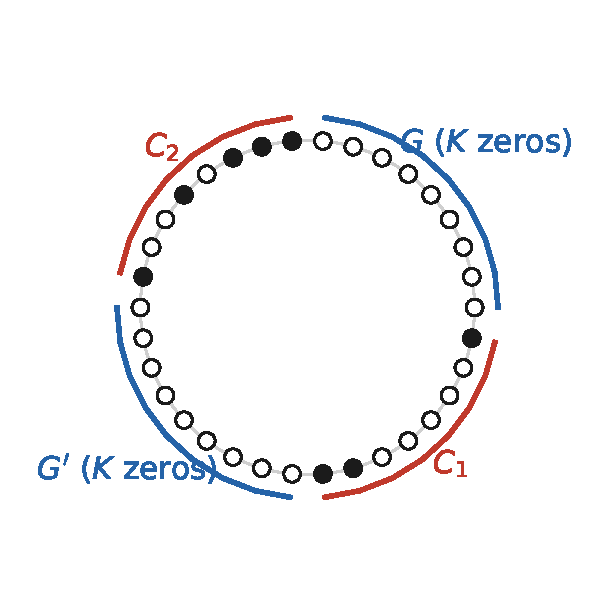
\includegraphics[width=0.55\textwidth]{fig_circle.pdf}
\caption{The anti-square $U_0 = V(9,1,1)$ read around a circle (filled: $1$, open: $0$). Two long gaps $G$ and $G'$ of $K=9$ zeros separate the clusters $C_1=1\,00000\,11$ and $C_2=1\,00\,1\,0\,111$. The proof compares how two copies would share the zeros of the long gaps: the eight short zeros in the clusters allow only a small imbalance, inequality~\eqref{eq:mass}.}
\label{fig:circle}
\end{figure}

Suppose, for a contradiction, that some rotation of $V$ is split into copies $A$ and $B$ spelling the same
word $u$. By Lemma~\ref{lem:split} each copy has $4\mu$ ones, so $u$ has $4\mu$ cyclic runs, which we index
modulo $4\mu$. Write $x_1, x_2, \alpha, \beta, \gamma$ for the numbers of zeros of $G, G', g_1, g_2, g_3$ in
$A$, so that $B$ has $y_1 = K\lambda - x_1$, $y_2 = K\lambda - x_2$, $5\lambda - \alpha$, $2\lambda - \beta$
and $\lambda - \gamma$ of them. Let $a$ be the number of ones of $A$ in $C_1$; then $B$ has $3\mu - a$ ones in
$C_1$ and $\mu + a$ in $C_2$, and exchanging the names of the copies replaces $a$ by $3\mu - a$. For a copy
$X$ that has a one in $C_2$, let $H_X$ and $T_X$ be the numbers of zeros of $X$ in $C_2$ before its first one
and after its last one there; define $H^1_X$ and $T^1_X$ in the same way for $C_1$. The zeros of $X$ in $C_2$
lying between two of its consecutive ones form its \emph{inner runs} in $C_2$, and similarly for $C_1$. For
example, if $X$ owns exactly the ones of $P_4$ and $P_5$ in $C_2$, then $H_X$ is its share of $g_2$,
$T_X = 0$, and its only inner run in $C_2$ that can be nonempty is its share of $g_3$, between the last one
of $P_4$ and the first one of $P_5$.

Two facts are used throughout. Both copies spell $u$, so each has half of the zeros:
\begin{equation}\label{eq:tot}
x_1 + x_2 + \alpha + \beta + \gamma = (K+4)\lambda .
\end{equation}
For each index $j$ let $m_A(j)$ be the number of zeros from $G$ and $G'$ in the $j$-th cyclic run of $A$,
define $m_B(j)$ likewise, and let $\sigma_A(j), \sigma_B(j)$ count the short zeros in these runs. Since
$m_A(j) + \sigma_A(j) = \rho_j = m_B(j) + \sigma_B(j)$, summing over $j$ gives
\begin{equation}\label{eq:mass}
\sum_{j} \lvert m_A(j) - m_B(j) \rvert \le 8\lambda .
\end{equation}

\subsection{Step 1: the long runs}
If $A$'s run spanning $G$ has index $i$, its run spanning $G'$ has index $i + a$, since $A$ passes $a$ of its
ones in between; likewise $B$'s two long runs have indices $j$ and $j + 3\mu - a$.

Suppose $0 < a < 3\mu$, so that each copy has two distinct long runs. Two coincidences between an index of $A$
and an index of $B$ would force either $i = j$ and $2a \equiv 3\mu$, which is impossible because $3\mu$ is
odd and $4\mu$ is even, or $j = i + a$ and $3\mu \equiv 0 \pmod{4\mu}$, also impossible. With no coincidence
the left side of~\eqref{eq:mass} is $2K\lambda$, and when the coincidence is on the same long gap it is at
least $K\lambda$; both exceed $8\lambda$. So $A$'s run spanning one long gap coincides with $B$'s run spanning
the other, and after exchanging the copies if necessary, $A$'s run $R$ spanning $G$ coincides with $B$'s run
$Q$ spanning $G'$. We call this \emph{type~T}.

If $a = 0$, the two long runs of $A$ are a single run, and by~\eqref{eq:mass} it coincides with one of the two
long runs of $B$. If $a = 3\mu$, exchanging the copies returns us to $a = 0$.

\subsection{Step 2: the case $a = 0$}
Here $B$ owns all of $C_1$ and $\mu \ge 1$ ones of $C_2$, and $A$'s long run has $T_A + x_1 + \alpha + x_2 +
H_A$ zeros. If it coincides with $B$'s run spanning $G'$, which has $y_2 + H_B = K\lambda - x_2 + H_B$ zeros,
then~\eqref{eq:tot} turns the equation into
\[
T_A + H_A + x_2 + 4\lambda = \beta + \gamma + H_B .
\]
The right side counts the zeros of $C_2$ held by $A$ together with those of $B$ before its first one
there, so it is at most $3\lambda$, a contradiction. If it coincides with $B$'s run spanning $G$, with $T_B + y_1$ zeros, the same
computation gives $T_A + H_A + x_1 + 4\lambda = \beta + \gamma + T_B \le 3\lambda$, again a contradiction.

\subsection{Step 3: type T}
The run $R$ has $T_A + x_1 + H^1_A$ zeros and $Q$ has $T^1_B + y_2 + H_B$. Equating them and
using~\eqref{eq:tot},
\begin{equation}\label{eq:RQ}
T^1_B + H_B + \alpha + \beta + \gamma = 4\lambda + T_A + H^1_A .
\end{equation}
Give $R$ and $Q$ the index $0$. Going forward, $A$ has its inner runs in $C_1$ at indices $1, \dots, a-1$, its
run $X_2$ spanning $G'$, with $T^1_A + x_2 + H_A$ zeros, at index $a$, and its inner runs in $C_2$ at
$a+1, \dots, 4\mu-1$. Likewise $B$ has its inner runs in $C_2$ at $1, \dots, \mu+a-1$, its run $Y_1$ spanning
$G$, with $T_B + y_1 + H^1_B$ zeros, at index $\mu+a$, and its inner runs in $C_1$ at
$\mu+a+1, \dots, 4\mu-1$. Matching runs index by index:
\begin{itemize}
\item[(c1)] at $1, \dots, a-1$, $A$'s inner runs in $C_1$ equal $B$'s first $a-1$ inner runs in $C_2$;
\item[(c2)] at $a$, $X_2$ equals $B$'s inner run between its $a$-th and $(a+1)$-th ones in $C_2$;
\item[(c3)] at $a+1, \dots, \mu+a-1$, $A$'s first $\mu-1$ inner runs in $C_2$ equal $B$'s inner runs there;
\item[(c4)] at $\mu+a$, $Y_1$ equals $A$'s inner run between its $\mu$-th and $(\mu+1)$-th ones in $C_2$;
\item[(c5)] at $\mu+a+1, \dots, 4\mu-1$, $A$'s remaining inner runs in $C_2$ equal $B$'s inner runs in $C_1$.
\end{itemize}
Sum (c1)--(c3) and (c3)--(c5), writing each total of inner runs as the zeros of that copy in the cluster less
its zeros before the first and after the last one, and add the two equations. With $F$ the total of the runs
in (c3), this gives
\begin{equation}\label{eq:inner}
H^1_A + T^1_B = 2\lambda + H_B + 2T_B + 2H_A + T_A + x_2 + y_1 + 2F .
\end{equation}
Since $C_1$ begins with $P_1$ and ends with $P_2$, we have $H^1_A = 0$ if $A$ owns a one of $P_1$, and
$H^1_A = \alpha$ otherwise; $T^1_B = 0$ if $B$ owns a one of $P_2$, and $T^1_B = 5\lambda - \alpha$ otherwise.
There are four branches.

If $A$ owns a one of $P_1$ and $B$ owns a one of $P_2$, the left side of~\eqref{eq:inner} is $0$, a
contradiction. If $A$ owns no one of $P_1$ but $B$ owns a one of $P_2$, then~\eqref{eq:RQ} reads $H_B + \beta
+ \gamma = 4\lambda + T_A$, while the left side is at most $3\lambda$. If $A$ owns a one of $P_1$ but $B$ owns no
one of $P_2$, then~\eqref{eq:RQ} reads $\lambda + H_B + \beta + \gamma = T_A$, while $T_A \le \beta + \gamma$.

In the last branch $A$ owns all of $P_2$ and none of $P_1$, so $a = 2\mu$. Then $A$'s inner runs in $C_1$ and
$B$'s inner runs in $C_1$ lie inside $P_2$ and $P_1$ and are empty, so (c1) says that $B$'s first $2\mu$ ones
in $C_2$ have no zeros of $B$ between them, and (c5) says the same of $A$'s last $\mu$ ones in $C_2$. Let $n_3,
n_4, n_5$ be the numbers of ones of $A$ in $P_3, P_4, P_5$, so that $n_3 + n_4 + n_5 = 2\mu$, and $B$ has
$2\mu - n_3 - n_4 = n_5$ ones in $P_3 \cup P_4$. In this branch $R = Q$ reads $T_A + x_1 + \alpha =
5\lambda - \alpha + y_2 + H_B$, and eliminating $\alpha$ with~\eqref{eq:RQ} gives
\begin{equation}\label{eq:last}
H_B + 2(\beta + \gamma) - T_A + x_2 - y_1 = 3\lambda .
\end{equation}
\begin{itemize}
\item If $1 \le n_5 < \mu$, then $B$'s first $2\mu$ ones in $C_2$ include a one before $g_3$ and a one after it,
  so $B$ has no zero of $g_3$ and $\gamma = \lambda$; but $A$'s last $\mu$ ones also straddle $g_3$, so
  $\gamma = 0$.
\item If $n_5 = 2\mu$, then $B$ owns $P_3$ and $P_4$, so (c1) gives $\beta = 2\lambda$, and $H_A = \beta + \gamma$.
  By (c2), $x_2 + H_A$ equals $B$'s run from the end of $P_4$ to its next one, which is $\lambda - \gamma$; that
  is, $x_2 + 2\lambda + 2\gamma = \lambda$.
\item If $\mu \le n_5 < 2\mu$ and $n_3 + n_4 < \mu$, then (c1) again gives $\gamma = \lambda$. The runs in (c3)
  on $B$'s side lie inside $P_5$, so $A$'s first $\mu$ ones in $C_2$ have no zeros of $A$ between them; they
  straddle $g_3$, so $\gamma = 0$.
\item If $n_3 + n_4 = \mu$ with $n_3, n_4 \ge 1$, then as before $\gamma = \lambda$ and $A$'s first $\mu$ ones
  have no zeros of $A$ between them, so $\beta = 0$; then (c4) gives $T_B + y_1 = \gamma$, so $y_1 = \lambda$,
  and (c2) gives $x_2 = H_A = 0$. Since $B$ owns a one of $P_3$ and $A$ a one of $P_5$, $H_B = T_A = 0$,
  and~\eqref{eq:last} reduces to $\lambda = 3\lambda$.
\item If $n_3 = 0$ and $n_4 = \mu$, then $B$'s first $2\mu$ ones in $C_2$ run from $P_3$ into $P_5$, so $\beta =
  2\lambda$; but (c2) forces $H_A = 0$, and $H_A = \beta$.
\end{itemize}
The remaining cases, $n_5 = 0$ and $(n_3, n_4) = (\mu, 0)$, give two splittings, and these satisfy every
equation between cyclic runs:
\begin{itemize}
\item[(S1)] $A$ owns $P_2$, $P_3$ and $\mu$ ones of $P_5$; $B$ owns $P_1$, $P_4$ and $2\mu$ ones of $P_5$; here
  $\gamma = \lambda$, $x_2 = 0$ and, by (c4), $y_1 = \beta + \lambda$.
\item[(S2)] $A$ owns $P_2$, $P_3$ and $P_4$; $B$ owns $P_1$ and $P_5$; here $x_2 = 0$ and $y_1 = \beta$.
\end{itemize}

\subsection{Step 4: the cut}
By Lemma~\ref{lem:split} the cut lies at a point of the circle covered by a run of $A$ and the run of $B$ with
the same index, and the two copies have equal numbers of zeros of that run after the cut. In both (S1)
and (S2) we have $y_1 \le 3\lambda$, so $x_1 \ge (K-3)\lambda \ge 6\lambda$.

At index $0$, $R$ runs from $A$'s last one in $C_2$ to the start of $P_2$, and $Q$ from the end of $P_1$ to
$B$'s first one in $C_2$. They overlap in $g_1$, and in (S2) also in $g_3$. A cut in $g_1$ leaves before it
all $x_1$ zeros of $G$ in $A$'s run but at most $5\lambda$ zeros in $B$'s, so the counts after the cut differ
as well. A cut in $g_3$ in (S2) leaves after it at most $\lambda$ zeros of $B$, but at least $x_1$ zeros of $A$.

At the other indices, in (S2) the runs of $A$ lie inside $P_2$ (indices $1$ to $2\mu-1$), span $G'$
(index $2\mu$), lie inside $P_3$, span $g_2$ (index $3\mu$) and lie inside $P_4$, while those of $B$ lie
inside $P_5$ (indices $1$ to $3\mu-1$), span $G$ (index $3\mu$) and lie inside $P_1$; no two with the same
index meet. In (S1) the runs of $A$ are the same up to index $3\mu - 1$, the run at $3\mu$ goes from the end of
$P_3$ to $A$'s first one of $P_5$, and the later ones lie inside $P_5$; those of $B$ lie inside $P_4$, then
run from $P_4$ to its first one of $P_5$ (index $\mu$), lie inside $P_5$, span $G$ (index $3\mu$) and lie
inside $P_1$. The only possible meeting is at index $3\mu$, when all of $B$'s ones in $P_5$ precede all of
$A$'s; then the two runs share only the point between $B$'s last one and $A$'s first one of $P_5$.
A cut at that point leaves no zero of $A$'s run after it but $y_1 + T_B \ge y_1 = \beta + \lambda > 0$ zeros
of $B$'s.

This completes the proof of Theorem~\ref{thm:blow}, and with $\lambda = \mu = 1$ and $K = k+9$, the proof that
$U_k$ is a shuffle anti-square. \qed

\section{The family $W_k$ and computer verification}\label{sec:verify}

The words $U_k$ cover the lengths $2n \ge 34$. For $24 \le 2n \le 32$ it suffices to exhibit one anti-square of
each length, which is a finite check: Grytczuk, Pawlik and Pleszczy\'nski list all of them for lengths $24$,
$26$ and $28$~\cite{GPP}, and $W_3$ and $W_4$ (lengths $30$ and $32$) pass the same exhaustive test. The family
$W_k$ covers every length at once: $W_0$ is their unique anti-square of length $24$, and $W_k$ is an
anti-square for every $k$.

For $W_k$ the reduction of Section~\ref{sec:runs} leaves one system of linear equations and inequalities in
$k$ and the shares $x_g$ for each cut gap and each way of dividing the twelve ones between the copies. There
are $12 \times 462$ such systems, and none has a solution, even over the reals with $k \ge 0$. We checked this
in three independent ways: by an exhaustive search over all rotations and splittings of $W_k$ for
$0 \le k \le 19$; with the SMT solver Z3 for the parametric systems; and in the Lean~4 proof assistant, where
we defined interleavings and shuffle squares from scratch, proved Lemma~\ref{lem:split} in the form of a
splitting relation on zero runs, and discharged every case with the linear-arithmetic procedure \texttt{omega}.
The Lean development proves, for every $n \ge 12$, that $W_{n-12}$ is an even word of length $2n$ none of whose
rotations is a shuffle square, and it depends on no axioms beyond propositional extensionality and quotient
soundness. It also proves the statement for $U_k$ independently of Section~\ref{sec:U}.

The exhaustive search reproduces the counts of~\cite{GPP} and extends them. Table~\ref{tab:counts} gives the
number of anti-squares up to rotation, reversal and exchange of the letters.

\begin{table}[h]
\centering
\begin{tabular}{lcccccc}
\toprule
length & 24 & 26 & 28 & 30 & 32 & 34 \\
\midrule
anti-squares & 1 & 26 & 103 & 660 & 2758 & 11026 \\
fewest ones & 12 & 10 & 10 & 10 & 8 & 8 \\
\bottomrule
\end{tabular}
\caption{Shuffle anti-squares by length (equivalence classes), and the smallest possible number of the rarer
letter.}\label{tab:counts}
\end{table}

\begin{remark}\label{rem:shape}
Both families have two long gaps, each longer than all the short gaps together, separating two clusters with an
odd number of ones. The parity argument of Section~\ref{sec:U} uses only this, while the short gaps do the rest;
the words $\zz{K}1^5\zz{K}1^7$ and $\zz{K}1^3\zz{K}1^5$, which have the same shape without short gaps, are not
anti-squares for any $K \le 20$ (by exhaustive check). It would be interesting to know the least number of ones in an anti-square of length $2n$ for
large $n$, and whether it stays bounded.
\end{remark}

\section{Cutting distance}\label{sec:cut}

In another paper~\cite{GPP2} the same authors measure how far an even word is from being a shuffle square by
cuts. Cutting a word into pieces and rearranging them gives another word with the same letters; let
$\operatorname{cut}(T, \mathcal{S}_2)$ be the least number of cuts that turns the even binary word $T$ into a
shuffle square, let $s(2, n)$ be its maximum over even binary words of length $n$, and let $s(2) = \sup_n s(2,
n)$. They conjectured that $s(2) = 1$~\cite[Conjecture 4]{GPP2}, having checked $s(2, n) \le 1$ for $n \le 20$.
With Ruci\'nski they later showed that an anti-square of length $24$ needs exactly two cuts, conjectured that
two cuts always suffice, that is $s(2) \le 2$, and noted that it is not even known whether $s(2)$ is
finite~\cite[Section 6.3]{GPR}.

One cut turns $T = PQ$ into $QP$, a rotation, so $\operatorname{cut}(T, \mathcal{S}_2) \le 1$ exactly when
some rotation of $T$ is a shuffle square. An anti-square therefore needs at least two cuts, and
Theorem~\ref{main} extends their example of length $24$ to every even length from $24$.

\begin{corollary}\label{cor:cut}
$s(2, 2n) \ge 2$ for every $n \ge 12$.
\end{corollary}

Their conjecture $s(2) \le 2$ holds for every anti-square we know. Two cuts split $T$ into $XYZ$, and apart
from rotations the rearrangements are $XZY$, $YXZ$ and $ZYX$. Testing these for every rotation of every
anti-square of length at most $34$, $1\,938\,732$ words in all, found a shuffle square each time. For
example, $W_0 = 0 \mid \zz{4}1 \mid \zz{2}1^4\zz{4}1^3 0\, 1^4$ rearranges as
$YXZ = \zz{4}1\,\zz{3}1^4\zz{4}1^3 0\, 1^4$, whose two copies both spell $\zz{2}1\zz{3}1^3 0\, 1^2$. For
$4 \le 2n \le 22$ there are no anti-squares, so $s(2, 2n) \le 1$, and the word $0110\,\zz{2n-4}$ is not
itself a shuffle square: its first letter precedes both ones, so $u$ begins with $0$ and each copy needs a
zero before its one, while only one zero precedes the ones. Hence $s(2, 2n) = 1$ for $4 \le 2n \le 22$ and
$s(2, 2n) = 2$ for $24 \le 2n \le 34$. Whether $s(2)$ is finite remains open.

\section*{Code and formal proof}
The programs, their outputs and the Lean~4 development are in the repository
\url{https://github.com/jvvk/mathematics}, in the folder \texttt{shuffle-anti-squares}. The Lean development, built on definitions of
interleavings, shuffle squares, rotations and cutting written from scratch, proves Theorem~\ref{main},
Theorem~\ref{thm:blow} with $K$, $\lambda$ and $\mu$ symbolic, Corollary~\ref{cor:cut}, the identity
$U_k = V(k+9,1,1)$, the splittings showing that both conditions of Theorem~\ref{thm:blow} are needed, and the
two-cut example of $W_0$ in Section~\ref{sec:cut}. Its proof of Theorem~\ref{thm:blow} does not follow
Section~\ref{sec:U} line by line: for each of the ten runs in which the cut can fall, it splits into cases on
which blocks of ones of the two copies overlap, and closes every case by linear arithmetic; a solver was used
only to choose the order of the case splits. The development depends on no axioms beyond propositional
extensionality, the axiom of choice and quotient soundness. Four statements rest on exhaustive computer search
and are not formalised: the counts in Table~\ref{tab:counts}, the absence of anti-squares below length $24$,
the claim that two cuts suffice up to length $34$ in Section~\ref{sec:cut}, and the check in
Remark~\ref{rem:shape}. Each was confirmed by a second program that shares no code with the first, and the
counts up to length $28$ also agree with the search of~\cite{GPP}.

\section*{Acknowledgements}
% VAMSHI: before journal submission, rewrite Sections 3 and 5 in your own words (EJC policy on AI-assisted
% proofs) and check every proof; then delete this comment.
The families $U_k$ and $W_k$ were found by computer search. The author used the AI assistant Claude
(Anthropic; Claude Opus 5.5 in October 2026 and earlier Claude models in September 2026) to write the search
and verification programs, to explore the case analysis, to find and draft the proof of
Theorem~\ref{thm:blow} and the observations of Section~\ref{sec:cut}, and to produce the Lean formalisation,
including the choice of case splits for Theorem~\ref{thm:blow}. It was used to search quickly and to obtain
machine-checked proofs: Theorems~\ref{main} and~\ref{thm:blow} and Corollary~\ref{cor:cut} are verified in
Lean, as described above. The author takes full responsibility for the content of this paper.

\begin{thebibliography}{9}
\bibitem{BV} L.~Bulteau and S.~Vialette, Recognizing binary shuffle squares is NP-hard,
\emph{Theoret. Comput. Sci.} 806 (2020), 116--132, doi:10.1016/j.tcs.2019.01.012.
\bibitem{GPP} J.~Grytczuk, B.~Pawlik and M.~Pleszczy\'nski, Variations on shuffle squares,
arXiv:2308.13882v2 (2024).
\bibitem{GPP2} J.~Grytczuk, B.~Pawlik and M.~Pleszczy\'nski, More variations on shuffle squares,
\emph{Symmetry} 15 (2023), 1982, doi:10.3390/sym15111982.
\bibitem{GPR} J.~Grytczuk, B.~Pawlik and A.~Ruci\'nski, Shuffle squares and ordered nest-free graphs,
arXiv:2503.22043v2 (2025); a shorter version appeared as Shuffle squares and nest-free graphs, in
\emph{Combinatorics on Words} (WORDS 2025), Lecture Notes in Comput. Sci., Springer, 2025, 166--178,
doi:10.1007/978-3-031-97548-6\_15.
\bibitem{HHNT} X.~He, E.~Huang, I.~Nam and R.~Thaper, Shuffle squares and reverse shuffle squares,
\emph{European J. Combin.} 116 (2024), 103883, doi:10.1016/j.ejc.2023.103883.
\bibitem{HP} X.~He and L.~Post, Asymptotically half of binary words are shuffle squares, arXiv:2512.12077
(2025).
\bibitem{HRS} D.~Henshall, N.~Rampersad and J.~Shallit, Shuffling and unshuffling,
\emph{Bull. Eur. Assoc. Theor. Comput. Sci.} 107 (2012), 131--142; arXiv:1106.5767.
\end{thebibliography}

\end{document}
